\chapter{FUNDAMENTAÇÃO TEÓRICA}

A implementação da nova Política Nacional de Segurança das Barragens (PNSB), instituída pela Lei nº 14.066, de 30 de setembro de 2020, estabeleceu marcos regulatórios fundamentais para o setor de mineração brasileiro, tornando compulsória a elaboração do Plano de Ação de Emergência (PAE) para todas as barragens destinadas à acumulação ou disposição de rejeitos de mineração \cite{brasil2020lei14066}.

Paralelamente, a Resolução ANM nº 40, de 6 de julho de 2020, determina que os empreendedores devem implementar sistemas de monitoramento de barragens em conformidade com a classificação do Dano Potencial Associado, estabelecendo prazo de 24 meses para a instalação dos equipamentos necessários \cite{anm2021resolucao56}. Além disso, a sofisticação do sistema de acompanhamento está condicionada à categorização do Dano Potencial Associado (DPA), o qual, quando classificado como elevado, onde há presença de população a jusante da estrutura com pontuação 10, bem como características construtivas que apresentem pontuação 10, demanda que esse controle seja contínuo e abrangente, cabendo à empresa a seleção da tecnologia, dos equipamentos e metodologias de monitoramento \cite{silva2019sistema}.

Conforme \cite{desouzajunior2018}, torna-se imprescindível que as estruturas de contenção possuam sistemas de acompanhamento e controle periódicos, visando antecipar comportamentos deformacionais nas barragens. Para \citeonline{castro2008}, além do acompanhamento sistemático, o próprio programa de monitoramento necessita de avaliação contínua, analisando seu desempenho e verificando se as condições estabelecidas estão sendo atendidas adequadamente. O autor ainda destaca que o projeto executivo bem estruturado constituirá o fundamento inicial para o monitoramento da barragem, devendo fornecer subsídios para que o responsável técnico avalie a eficácia da instrumentação implementada e determine quando serão necessários ajustes.

A norma ABNT NBR 13028, em seus requisitos para elaboração e apresentação de projetos, especificamente no capítulo 5.4.16, item "i", estabelece que deve ser considerado o manual operacional da estrutura, contemplando procedimentos de inspeção in loco e monitoramento. Quanto ao monitoramento, a norma determina que sejam especificados os componentes a serem acompanhados, a periodicidade das inspeções de campo, as leituras instrumentais e os parâmetros de análise dos dados coletados \cite{abnt2017}.

Dessa forma, evidencia-se que o monitoramento eficaz das barragens de mineração fundamenta-se nas inspeções de campo, executadas por equipe técnica especializada, e nas informações de variáveis que subsidiam as decisões relacionadas à integridade estrutural. Diversos pesquisadores como \citeonline{machado2007}, \citeonline{castro2008} e \citeonline{soares2010} indicam em seus estudos que os principais parâmetros a serem monitorados nas barragens relacionam-se às diferentes modalidades de entrada e saída de água do reservatório, as quais evidenciarão as variações hidrostáticas das estruturas e, consequentemente, sua estabilidade. Tais informações essenciais são obtidas mediante sistema de instrumentação instalado nas barragens de mineração, auxiliando no processo decisório e apresentando o estado real das estruturas.

\section{A relevância da Instrumentação de barragens de mineração}

O processo de instrumentação das estruturas, conforme destacado por \cite{fonseca2003auscultacao}, possibilita a execução sistemática de aquisição, registro e processamento detalhado de informações coletadas através dos dispositivos de medição instalados em distintas seções e zonas das barragens. As avaliações contemplam os parâmetros limite de cada ponto observado no programa de instrumentação, visando acelerar a identificação de possíveis anomalias. Dessa forma, um programa de instrumentação objetiva assegurar precisão e disponibilizar parâmetros associados à confiabilidade das medições e correspondência entre os critérios projetuais e a metodologia executiva.

Segundo \cite{machado2007}, visando minimizar os riscos de acidentes em empreendimentos de barragens, considerando os impactos gerados por tais ocorrências, justifica-se a preocupação atual em instrumentar barragens utilizando tecnologia moderna e, quando viável, nacional. Por meio da instrumentação, identificam-se pontos nas barragens onde existem níveis críticos de segurança estrutural e operacional. A segurança estrutural apresenta maior relevância, uma vez que compromete a estabilidade da barragem. A segurança operacional relaciona-se ao funcionamento dos equipamentos da barragem, como medidores de vazão.

Conforme \cite{machado2007}, apesar da grande ênfase atribuída à segurança, a instrumentação de barragens possui como objetivo fundamental a obtenção de redução global nos custos do empreendimento. A instrumentação possibilita trabalhar com margem de segurança adequada, dispensando segurança adicional desnecessária, o que resultaria em elevação dos custos financeiros da obra.

Observa-se que a utilização de instrumentos para monitoramento de barragens de mineração demanda projeto bem fundamentado, além de programa de instrumentação que deve constituir mecanismo dinâmico para acompanhamento e análise dos dados. A Figura \ref{fig:rotina_instrumentacao} apresenta, esquematicamente, os principais elementos da rotina de um projeto de instrumentação \cite{machado2007}.

\begin{figure}[htbp]
    \centering
    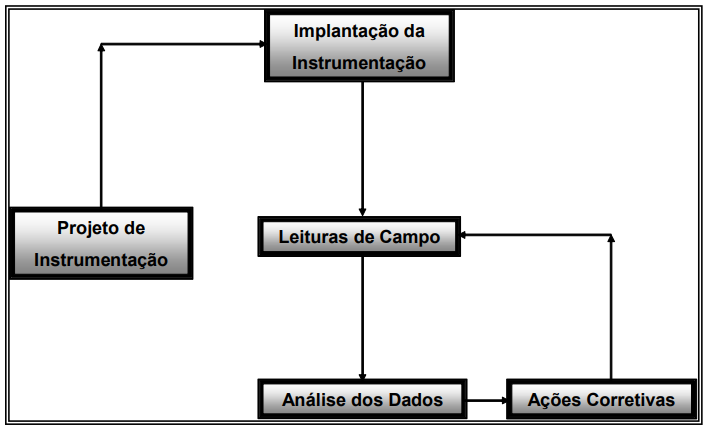
\includegraphics[width=0.8\textwidth]{figures/image39_rotina_instrumentacao_barragem.png}
    \caption{Rotina de um programa de instrumentação de barragem.}
    \fonte{\cite{machado2007}}
    \label{fig:rotina_instrumentacao}
\end{figure}

A instrumentação, mediante informações obtidas através da realização de leituras, complementa as inspeções visuais de barragens e garante o monitoramento das medições de deslocamento, pressão, percolação e drenagem, além de outros fatores que influenciam o comportamento da estrutura, como nível do reservatório e precipitação \cite{machado2007}.

\section{Instrumentação para Barragens de Rejeito}

Torna-se imprescindível o acompanhamento da evolução comportamental dessas estruturas ao longo do tempo, demandando a instalação de instrumentos adequados para o monitoramento, proporcionando leituras dos parâmetros mais significativos relacionados ao seu desempenho \cite{machado2007}.

As metodologias de auscultação comportamental de barragens abrangem a seleção tipológica e a quantificação dos instrumentos a serem empregados, seu posicionamento e instalação, a coleta de dados (automatizada ou baseada em leituras periódicas realizadas por equipe capacitada), análise e interpretação dos resultados. Este conjunto de metodologias constitui o denominado sistema de instrumentação geotécnica, sendo objeto de considerável interesse e desenvolvimento no Brasil nos últimos anos \cite{machado2007}.

O programa de instrumentação objetiva principalmente a adequação do monitoramento da estrutura aos parâmetros necessários para acompanhamento da integridade da barragem, devendo constituir um mecanismo ativo e constantemente reavaliado \cite{silva2019sistema}. As etapas de um programa de monitoramento são apresentadas de forma resumida na Figura \ref{fig:fases_programa_monitoramento}.

\begin{figure}[htbp]
    \centering
    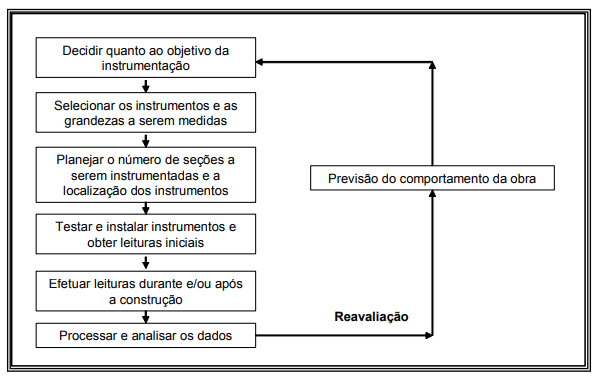
\includegraphics[width=0.8\textwidth]{figures/image40_fases_programa_monitoramento.png}
    \caption{Fases de um programa de monitoramento.}
    \fonte{\cite{machado2007}}
    \label{fig:fases_programa_monitoramento}
\end{figure}

A instrumentação de auscultação implementada em barragens de rejeitos objetiva avaliar o comportamento real dos rejeitos quanto ao desenvolvimento de deformações e pressões intersticiais, obter dados de deslocamento, tensão total, vazão, nível d'água e comparar estes dados coletados através de leituras periódicas aos respectivos valores de controle, máximo e mínimo, especificados nos critérios de projeto. Os relatórios dos programas de inspeção e instrumentação devem ser analisados tecnicamente de forma a possibilitar a adoção de ações efetivas imediatas, quando necessário \cite{machado2007}.

Os principais dados monitorados pelos instrumentos referem-se à piezometria, vazão de jusante, pluviometria, nível de água do reservatório e os marcos topográficos superficiais. Conforme já mencionado, tais informações apresentarão principalmente o comportamento da variação hídrica no reservatório e nas estruturas, além da capacidade da barragem em absorver, drenar e vertê-la para jusante \cite{silva2019sistema}. A figura \ref{fig:formas_entrada_saida_agua_barragens} apresenta genericamente os principais mecanismos de entrada e saída de água dos reservatórios das barragens de mineração.

\begin{figure}[htbp]
    \centering
    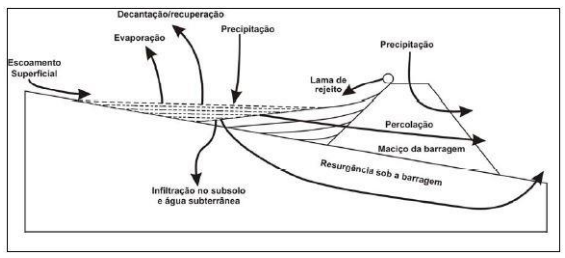
\includegraphics[width=0.8\textwidth]{figures/image41_formas_entrada_saida_agua_barragens.png}
    \caption{Formas de entrada e saída de água das barragens.}
    \fonte{\cite{silva2019sistema}}
    \label{fig:formas_entrada_saida_agua_barragens}
\end{figure}

\subsection{Instrumentação para medições do comportamento do nível d'água}

A determinação da posição da linha freática constitui elemento essencial para estudos relacionados ao comportamento geotécnico de estruturas de contenção. O sistema de monitoramento das manifestações hidráulicas caracteriza-se, fundamentalmente, como um dispositivo destinado ao registro permanente dos níveis de água, estabelecendo limites críticos que desencadeiam alertas e implementação de medidas preventivas para correção de eventuais anomalias \cite{machado2007}.

Os equipamentos piezométricos têm sido extensivamente empregados no acompanhamento e análise preditiva do comportamento de inúmeras barragens mundialmente \cite{machado2007}. A oscilação dos dados piezométricos pode manifestar-se mediante a ocorrência de uma das seguintes situações: incremento da vazão de percolação; elevação dos níveis d'água à montante e jusante; ampliação da permeabilidade dos materiais situados à montante do piezômetro; diminuição da permeabilidade dos materiais posicionados à jusante do piezômetro \cite{machado2007}.

Constituem instrumentos que viabilizam a mensuração dos níveis piezométricos na interface maciço/fundação, proporcionando uma análise dos parâmetros de subpressão estabelecidos no dimensionamento. Tais instrumentos podem ser posicionados em distintas profundidades à jusante da estrutura \cite{machado2007}.

Dentre os modelos de equipamentos disponibilizados comercialmente, destacam-se os mais empregados: Medidor de nível d'água, Tubo aberto (standpipe), Pneumáticos, Hidráulicos, Elétricos e de Corda Vibrante \cite{machado2007}. No presente trabalho será enfatizado o modelo de medidor de nível d'água, razão pela qual será apresentado subsequentemente.

\subsubsection{Medidor de Nível d'água}

Uma das metodologias para mensurar a saturação do solo consiste na utilização de um medidor de nível d'água. Este dispositivo caracteriza-se por um tubo perfurado inserido no solo até alcançar o lençol freático, similarmente a um poço. Desta maneira, torna-se imprescindível o conhecimento prévio das características do terreno para determinar a profundidade adequada de inserção \cite{victorino2003piezometro}.

Conforme descrito por \cite{victorino2003piezometro}, o sistema instalado no terreno é constituído utilizando-se:

\begin{enumerate}
\item Tubo de PVC, com perfurações preparadas ao longo de sua extensão;
\item Conexões do tubo, tampas superior e inferior;
\item Areia lavada para constituir um filtro ao redor do tubo;
\item Geotêxtil, que favorece exclusivamente a passagem de água para o interior do tubo;
\item Bentonita ou cimento para vedação do sistema.
\end{enumerate}

O equipamento, de baixo investimento, possivelmente o instrumento mais elementar de construir e operar, permite que no interior do tubo seja armazenada somente a água correspondente ao nível do lençol freático e demais aquíferos presentes no terreno \cite{victorino2003piezometro}. Um esquema do mesmo encontra-se representado na Figura \ref{fig:sistema_medidor_dagua}.

\begin{figure}[htbp]
    \centering
    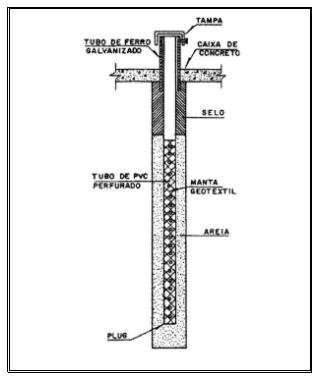
\includegraphics[width=0.8\textwidth]{figures/image43_sistema_medidor_dagua.png}
    \caption{Sistema com tubo para medir o nível d'água.}
    \label{fig:sistema_medidor_dagua}
    \fonte{\cite{victorino2003piezometro}}
\end{figure}

Para \cite{fonseca2003auscultacao}, a informação referente ao nível do lençol freático no interior das estruturas da barragem é indispensável para execução das análises de estabilidade ou para interpretação dos resultados piezométricos. A aplicação destes instrumentos para mensuração de nível de água das estruturas fundamenta-se em acessar diretamente a água em profundidade e realizar a medição da cota da superfície. Usualmente o acesso à água é executado por meio de métodos simples como sondagem ou perfurações de trado, e na medição da cota utiliza-se comumente um cabo graduado que possui um sensor na extremidade inferior e que emite um sinal sonoro e luminoso ao alcançar a água.

A mensuração é executada normalmente de forma manual, com uma escala ou equipamento, visualizado na Figura \ref{fig:indicador_nivel_dagua}, que identifique a superfície da água no interior do tubo, que no caso deste instrumento corresponderá sempre, precisamente, ao nível freático \cite{machado2007}.

\begin{figure}[htbp]
    \centering
    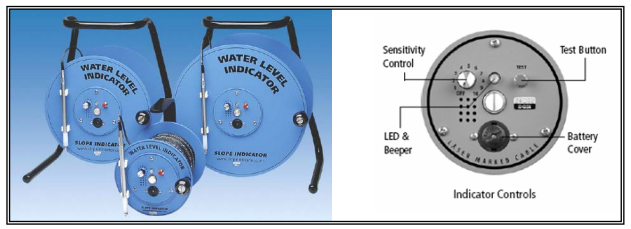
\includegraphics[width=0.6\textwidth]{figures/image44_indicador_nivel_dagua.png}
    \caption{Indicador de nível d'água.}
    \label{fig:indicador_nivel_dagua}
    \fonte{\cite{machado2007}}
\end{figure}

\subsection{Instrumentação para medições de deslocamentos}

As barragens de terra e rejeitos encontram-se continuamente expostas a deslocamentos e deformações, decorrentes de suas características intrínsecas e dimensões, bem como de fatores internos e externos. Nesse contexto, torna-se fundamental aprofundar o estudo desse fenômeno e a aplicação de metodologias e tecnologias inovadoras que possam auxiliar no monitoramento dessas estruturas \cite{machado2007}.

A quantificação de deslocamentos e deformações representa a sistematização das observações acerca do comportamento estrutural, constituindo uma prática de crescente relevância na atualidade. Tal importância deriva das dimensões que as barragens de rejeitos alcançam mediante alteamentos sucessivos, reflexo do incremento da produção mineira, resultando em maior volume de rejeitos e, consequentemente, reforçando a significância dessas medições \cite{machado2007}.

As principais dificuldades relacionam-se, de modo geral, com a mensuração de deformações e deslocamentos horizontais, bem como distorções. Nas décadas recentes, observou-se um crescimento considerável não apenas no número, mas também na altura das barragens. Por essa razão, intensificaram-se as exigências por qualidade e precisão nos métodos de instrumentação e auscultação \cite{machado2007}.

\subsubsection{Inclinômetro}

Os inclinômetros são empregados com a finalidade de quantificar deformações e deslocamentos horizontais em massas de solo, além de identificar regiões com concentração de deformações, ou seja, superfícies potenciais de ruptura. Estes instrumentos apresentam particular adequação para tal aplicação, uma vez que as medições são realizadas no interior da massa de solo \cite{machado2007}.

O funcionamento do equipamento ocorre da seguinte maneira: o inclinômetro é constituído por uma haste cilíndrica contendo um sensor de inclinação incorporado em seu interior e duas ou quatro rodas distribuídas lateralmente. As rodas se ajustam às ranhuras presentes em um tubo flexível instalado no solo, permitindo que o sensor acompanhe a orientação do tubo. Procede-se então à medição da inclinação do tubo em intervalos regulares, calculando-se, a partir do ângulo de inclinação, o deslocamento de cada segmento tubular. O tubo é normalmente instalado no furo de sondagem, sendo realizadas medições de deslocamento ao longo do tempo para monitorar a movimentação do solo \cite{dunnicliff1988geotechnical}. A Figura~\ref{fig:inclinometro_funcionamento} ilustra seu funcionamento.

\begin{figure}[htbp]
    \centering
    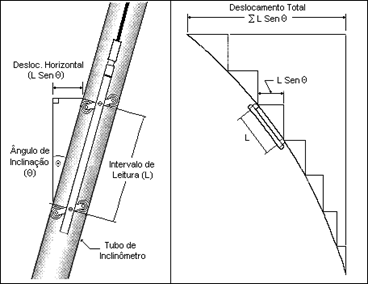
\includegraphics[width=0.8\textwidth]{figures/image45_representacao_funcionamento_inclinometro.png}
    \caption{Representação do funcionamento de um inclinômetro.}
    \label{fig:inclinometro_funcionamento}
    \fonte{\cite{dunnicliff1988geotechnical}}
\end{figure}

\subsection{Instrumentação para medições hidrológicas}

Informações hidrológicas, incluindo precipitação, pluviometria e precipitação média regional, viabilizam a análise tanto da bacia de interesse quanto de bacias situadas a jusante. O conhecimento das características pluviométricas constitui elemento fundamental para a hidrologia, especialmente no dimensionamento de vertedores em estruturas de barragens.

A quantificação da variável precipitação pode ser realizada de forma pontual mediante a utilização de dois equipamentos meteorológicos: o pluviômetro e o pluviógrafo. A distinção principal entre estes instrumentos reside no fato de que o pluviógrafo efetua o registro automático das informações, enquanto o pluviômetro demanda leituras manuais em intervalos temporais predefinidos.

\subsubsection{Instituto Nacional de Meteorologia (INMET)}

O Instituto Nacional de Meteorologia (INMET), órgão vinculado ao Ministério da Agricultura e Pecuária, tem como missão institucional promover e coordenar atividades destinadas à produção de informações meteorológicas oportunas e relevantes, visando a mitigação de riscos e o desenvolvimento sustentável do setor agropecuário, a conservação ambiental e a segurança da sociedade brasileira \cite{inmet2025sobre}.

Entre as principais competências do INMET destacam-se o monitoramento das condições meteorológicas e climáticas, a elaboração de previsões meteorológicas e climáticas, a emissão de alertas de tempo severo e a disponibilização de diversos produtos de apoio ao setor agrícola, incluindo atividades de pesquisa e desenvolvimento \cite{inmet2025sobre}.

O Sistema de Coleta e Distribuição de Dados Meteorológicos da instituição (temperatura, umidade relativa do ar, direção e velocidade do vento, pressão atmosférica, precipitação, entre outras variáveis) é constituído por estações meteorológicas de superfície operando continuamente; além da maior rede de estações automáticas da América do Sul \cite{inmet2025sobre}.

Este órgão realiza o monitoramento e análise das previsões meteorológicas, fornecendo informações detalhadas sobre índices pluviométricos nos estados brasileiros. A plataforma digital do INMET disponibiliza informações relevantes que contribuem para alertas preventivos e adequados sobre riscos de desastres naturais. Complementarmente aos alertas, são divulgados no portal dados referentes ao início e término dos eventos, grau de severidade dos fenômenos, além das medidas preventivas recomendadas à população \cite{inmet2025sobre}.

Adicionalmente, é possível obter através da plataforma do INMET informações sobre o acúmulo pluviométrico nas últimas 24 horas em diversas regiões do território nacional. A Figura \ref{fig:precipitacao_24h} apresenta um exemplo de mapeamento de precipitação referente ao dia 28/04/2025 \cite{inmet2025precipitacao}.

\begin{figure}[htbp]
    \centering
    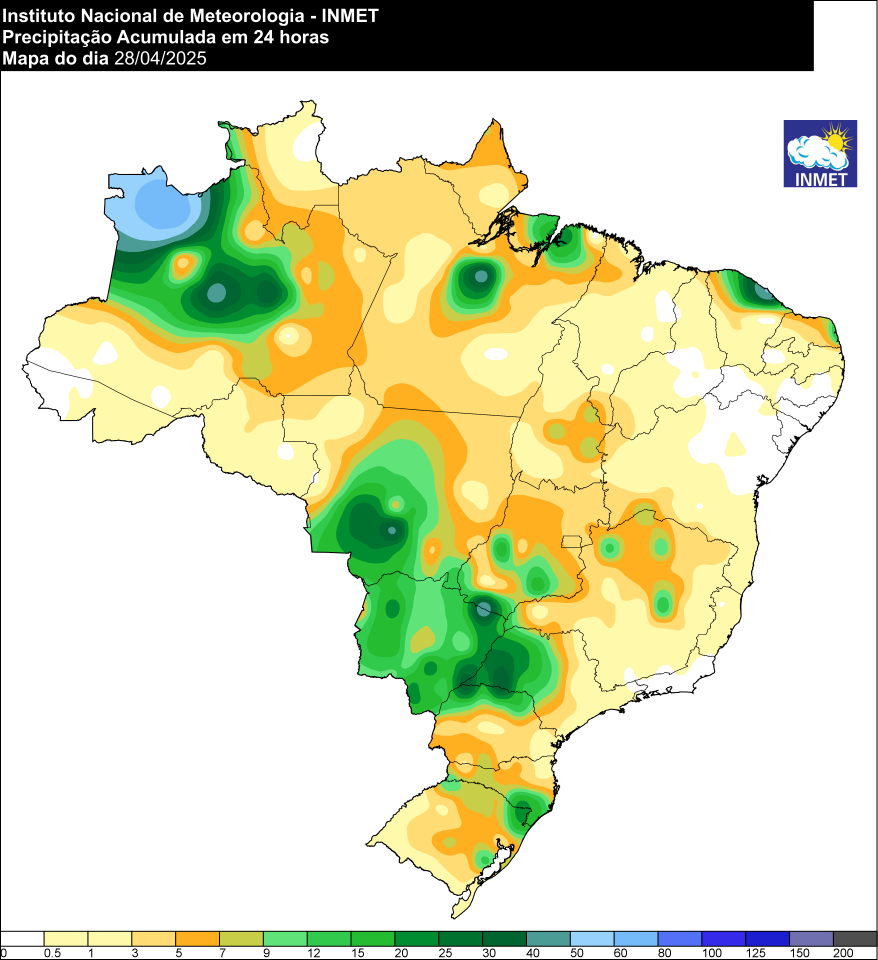
\includegraphics[width=0.8\textwidth]{figures/image46_precipitacao_acumulada_24h.png}
    \caption{Mapeamento de precipitação referente ao dia 28/04/2025.}
    \label{fig:precipitacao_24h}
    \fonte{\cite{inmet2025precipitacao}}
\end{figure}

Outra metodologia para análise da precipitação de determinada localidade através dos dados disponibilizados pelo INMET consiste na utilização de tabelas que indicam a taxa pluviométrica (mm/h) em local específico para o período desejado, complementadas por informações de temperatura (°C), umidade (%), ponto de orvalho (%), pressão (hPa), vento (m/s) e radiação (kJ/m²). A Figura \ref{fig:dados_inmet} apresenta uma tabela deste modelo para o município de Ibirité, Minas Gerais, em um intervalo temporal que se estende das 00:00 horas do dia 28/04/2025 até as 21:00 horas do dia 30/04/2025 \cite{inmet2025estacao}.

\begin{figure}[htbp]
    \centering
    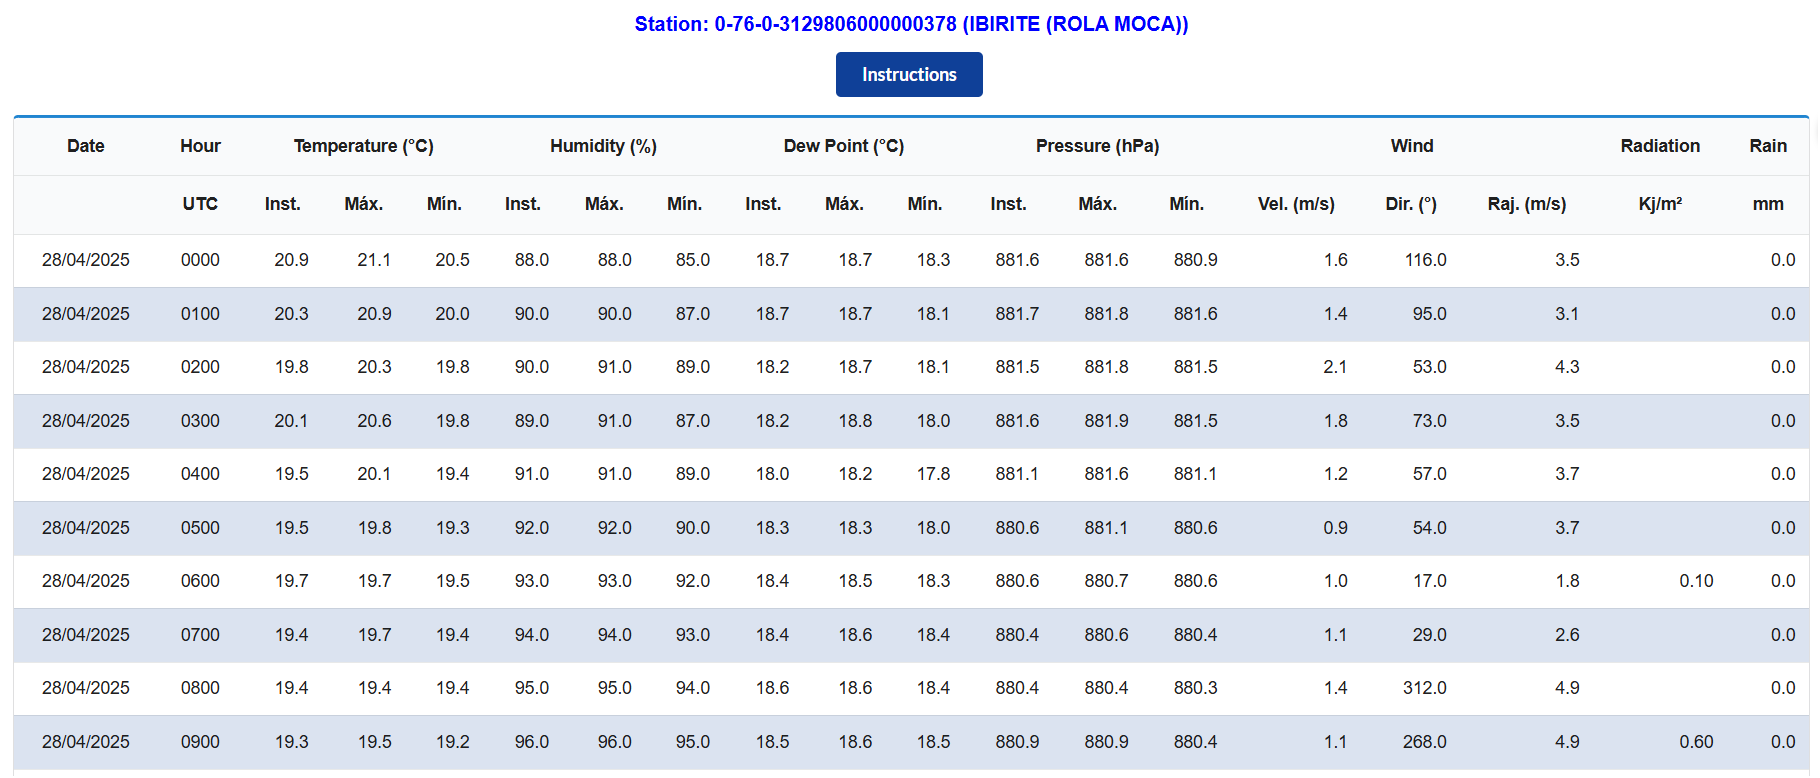
\includegraphics[width=0.8\textwidth]{figures/image47_principais_dados_mensurados_inmet.png}
    \caption{Principais dados meteorológicos mensurados pelo INMET para Ibirité, MG.}
    \label{fig:dados_inmet}
    \fonte{\cite{inmet2025estacao}}
\end{figure}

\section{Automação da Instrumentação}

Em projetos geotécnicos de grande escala, os sistemas de instrumentação e monitoramento constituem elementos fundamentais para a identificação de pontos críticos relacionados à segurança estrutural e operacional. A implementação de sistemas automatizados de monitoramento e instrumentação dessas estruturas proporciona à equipe técnica responsável pela gestão dos dados das barragens acesso às informações da instrumentação em tempo real. Consequentemente, o processo se torna mais eficiente, proporcionando maior agilidade na interpretação dos dados e, por conseguinte, maior confiabilidade no processo decisório. Ademais, a automação das barragens possibilita o incremento da frequência de leituras e elimina a necessidade de coleta manual dos dados por profissional especializado \cite{chammas2016monitoramento}.

Com o desenvolvimento tecnológico, o conceito de automatização emergiu na área de instrumentação de barragens. Para os instrumentos mais empregados nestes empreendimentos, tais como indicadores de nível de água, piezômetros, inclinômetros e marcos superficiais, existem suas respectivas versões automatizadas, as quais devem ser utilizadas tanto na fase construtiva quanto na operacional da barragem. A adequada leitura e interpretação dos resultados produzidos pela instrumentação permite verificar as condições que determinam a estabilidade da barragem, estabelecendo níveis de alarme para atuações de caráter preventivo. O desenvolvimento de microcontroladores, dataloggers e, dentre outros, a transmissão de dados via rádio, fibra ótica e até comunicação satelital propiciaram um sistema de automatização da instrumentação de barragens. Com a evolução das tecnologias para instrumentação, foram alcançados avanços significativos relacionados à coleta de dados, transmissão, processamento e análise de informações \cite{quispe2018instrumentacao}.

Ainda conforme \cite{quispe2018instrumentacao}, os instrumentos automatizados garantem confiabilidade para aquisição dos dados, contudo, existe um custo substancial para implementação e previsão de retorno a longo prazo.

Segundo \cite{machado2007}, em contrapartida ao sistema convencional, o sistema com instrumentação automática pode apresentar falhas nos sensores e nos equipamentos eletrônicos devido à sua sensibilidade perante as condições reais de operação em campo.

O monitoramento automático é executado através de um conjunto de equipamentos eletrônicos constituindo um sistema programável, no qual as tarefas de medição e controle são desempenhadas. A este denomina-se sistema de aquisição e transmissão automática de dados (SATAD). Os dados de cada instrumento são enviados ao SATAD e este, por sua vez, transmite as informações para um Centro de Controle onde os dados são processados e avaliados pela equipe competente. Nesta central é realizada a gestão dos dados com o auxílio de um programa de controle que pode armazenar e organizar as informações recebidas. Além disso, este programa possui as funcionalidades de indicar o status atual de segurança vigente para cada instrumento ou conjunto deles, possibilidade de modificação da frequência das leituras, geração de relatórios, emissão de alertas sonoros e visuais \cite{machado2007}.

O monitoramento inicial constitui o período no qual são ajustados os instrumentos, verificam-se as discrepâncias de calibração dos mesmos, analisados os instrumentos inoperantes e ajustado o sistema de automação. Esta representa uma das fases mais importantes no processo, quando então são coletados os dados, razão pela qual a supervisão e manutenção do sistema de monitoramento devem ser realizadas com total atenção e zelo \cite{machado2007}.

A verificação em campo torna-se necessária quando existem dúvidas sobre valores que ultrapassam os limites sem, aparentemente, observar anomalias na estrutura. Para que seja possível identificar comportamentos anômalos tanto das estruturas quanto dos próprios instrumentos, é importante que exista uma definição de faixas de valores aceitáveis para cada instrumento \cite{machado2007}.

Segundo \cite{machado2007}, as duas modalidades de obtenção de dados da instrumentação são utilizadas, sendo:

\begin{itemize}
    \item \textbf{Aquisição Manual:} sistema tradicional de coleta de dados, utilizado em diversas barragens. Os dados, após terem sido coletados manualmente através de instrumentos de leitura visual pelo técnico, são transcritos em tabelas para serem, posteriormente, interpretados e apresentados sob forma de gráfico;
    
    \item \textbf{Aquisição Automatizada:} o sistema automático constitui uma prática amplamente difundida atualmente. Este sistema oferece um número considerável de medidas ao longo do dia. Neste processo evitam-se erros de leitura obtidos por leitura manual.
\end{itemize}

E ainda segundo \cite{machado2007}, as principais grandezas comumente monitoradas em barragens de terra e rejeito são:

\begin{itemize}
    \item Deslocamentos;
    \item Deformações e tensões;
    \item Níveis piezométricos em fundação;
    \item Pressões de água;
    \item Vazão.
\end{itemize}

Os instrumentos mais comuns são os marcos superficiais, os inclinômetros, os piezômetros, os deformímetros e estações meteorológicas \cite{machado2007}. A Figura \ref{fig:instrumentacao_barragem_terra} apresenta o mapeamento dos principais locais e instrumentos possíveis de serem instalados em barragem de terra.

\begin{figure}[htbp]
    \centering
    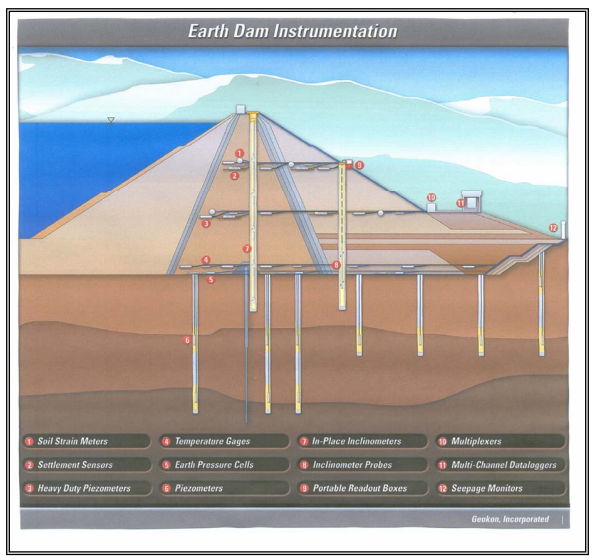
\includegraphics[width=0.8\textwidth]{figures/image42_instrumentacao_barragem_de_terra.png}
    \caption{Instrumentação em barragem de terra.}
    \label{fig:instrumentacao_barragem_terra}
    \fonte{\cite{machado2007}}
\end{figure}

\subsection{Dataloggers}

O \textit{datalogger} constitui um equipamento eletrônico composto por um microcontrolador e um voltímetro com memória. Este dispositivo possui as funcionalidades para realizar diversas tarefas como produzir tensão pré-estabelecida com intervalos definidos, ler tensões e também para armazenar dados. Além disso, pode ser configurado para executar cálculos e armazenar os resultados, como por exemplo, converter a leitura de um piezômetro para diferentes unidades. Os instrumentos são interligados às conexões ou às denominadas "portas" no equipamento e a coleta de leitura é realizada em intervalos selecionados. Dispositivos periféricos podem ser interligados às portas de controle e de excitação para executar funções específicas, como telefonia celular e testadores de cabo. Os dataloggers interligados à instrumentação eletrônica podem executar tarefas distintas automaticamente, como em determinado nível de alarme de um sensor ativar uma ação, como alarme luminoso ou sirene \cite{kane2000instrumentation}.

De acordo com \cite{cerqueira2016estudo}, o \textit{datalogger} constitui o principal componente de uma estação de campo para automatização da instrumentação de uma barragem. Este dispositivo tem por finalidade receber, armazenar e converter os dados de campo. Com a interligação dos instrumentos a este equipamento, é possível realizar a programação para registro contínuo das leituras dos piezômetros eliminando a necessidade de coleta periódica manual dos instrumentos. \cite{santos2012utilizacao} complementa que os \textit{dataloggers} podem também realizar a medição desejada periodicamente em intervalo pré-definido e estas serem salvas em um banco de dados interno. Sendo necessário, de acordo com o grau de automação, a conexão e extração destes dados no equipamento. A Figura \ref{fig:datalogger_automacao} apresenta um exemplo de um \textit{datalogger} frequentemente utilizado em projetos para automação de barragens de mineração.

\begin{figure}[htbp]
    \centering
    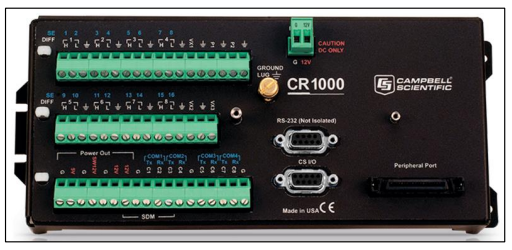
\includegraphics[width=0.6\textwidth]{figures/image48_datalogger_usada_automacao_barragens.png}
    \caption{\textit{Datalogger} utilizado em sistemas de automação de barragens.}
    \label{fig:datalogger_automacao}
    \fonte{\cite{inmet2025estacao}}
\end{figure}

Na maior parte das aplicações, os dataloggers constituem parte de uma solução de automação e são interligados via rede para a aquisição dos dados por eles coletados. São instalados próximos aos sensores e os resultados são armazenados em formato de arquivo e compartilhados com estações servidoras remotas nas quais possuem softwares proprietários capazes de interpretar, plotar gráficos e realizar novas configurações nestes equipamentos \cite{silva2019sistema}.